% classical.tex

% take classification as a case study
\begin{frame}
    \frametitle{(Supervised) Classification Problem}

    Given a set of input vectors with labels \({\vec{x_i}, y_i}\), learn a
    model, and attempt to predict the labels for arbitrary inputs.

    % add diagram TODO
    \begin{figure}
        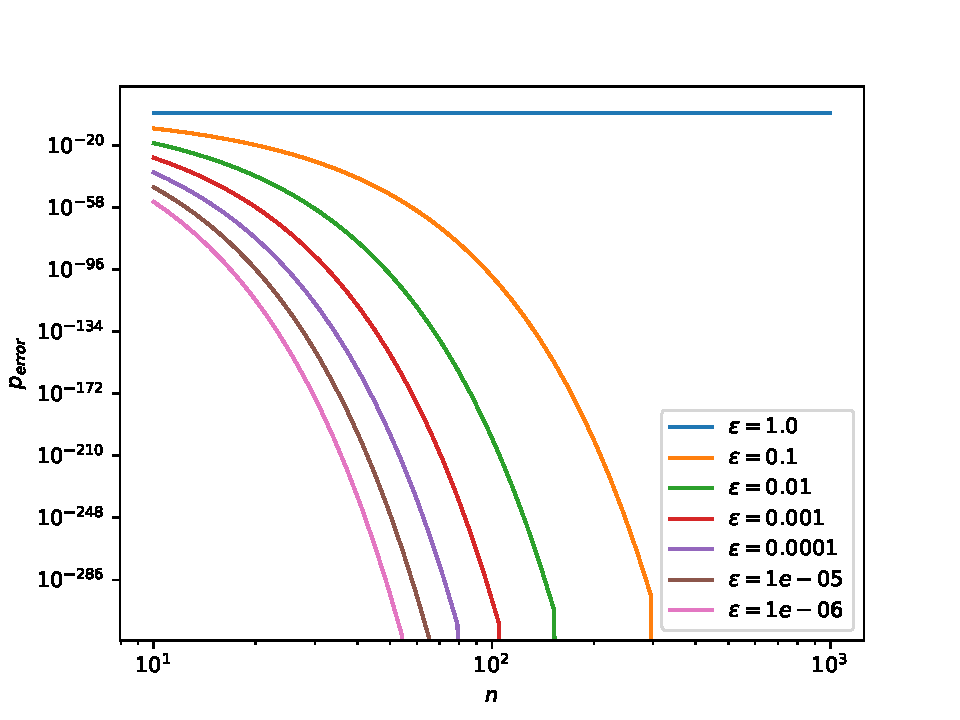
\includegraphics[width=0.6\textwidth]{figures/perrorplot.pdf}
    \end{figure}

\end{frame}

% svm
\begin{frame}
    \frametitle{Support Vector Machines (SVM)}

    Support Vector Machine or Maximum Margin Classifier attempts to find a
    separating plane between labels and optimizes the margin, i.e., distance
    from inputs on either side to it.

    \begin{multicols}{2}
        % svm fig
        \begin{figure}
            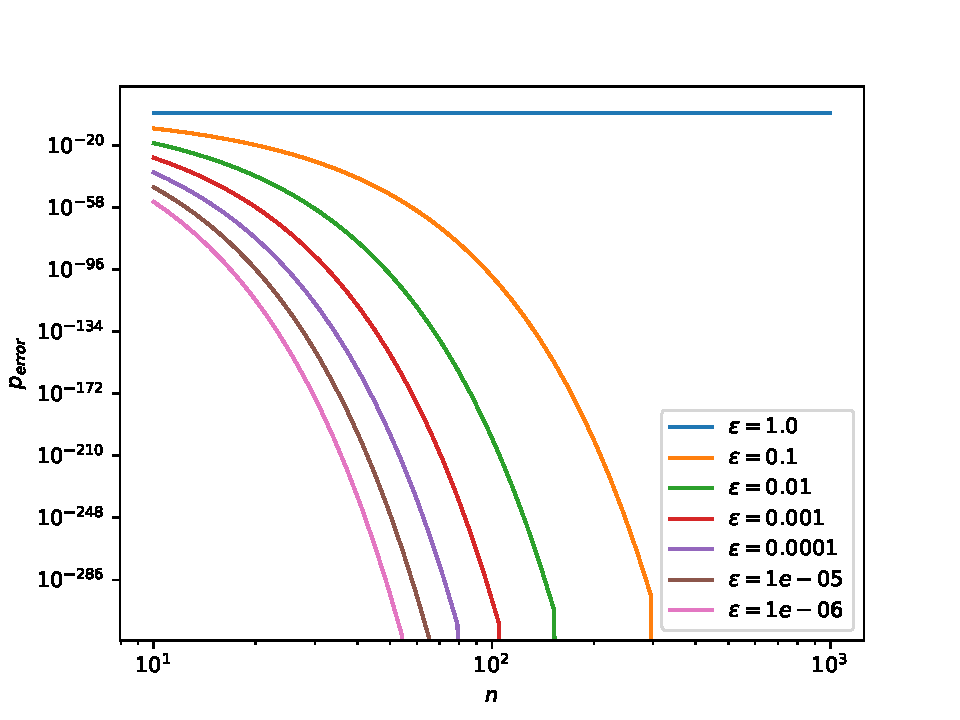
\includegraphics[width=0.5\textwidth]{figures/perrorplot.pdf}
        \end{figure}
        %
        Hyperplane characterized by a normal vector and a bias \((\vecw, b) \in
        \reals^{n+1}\).
        \begin{gather*}
            \innerproductabstract{\vecw}{\vec{x_i}} + b \geq 1 \text{ if } y_i = 1~, \text{and}\\
            \innerproductabstract{\vecw}{\vec{x_i}} + b \leq -1 \text{ if } y_i = -1~.
        \end{gather*}

        We minimize

        \begin{equation*}
            \mathcal{L}(\vecw, \vec{\alpha}) = \frac{1}{2} \innerprod{\vecw}{\vecw} + \sum_i \alpha_i \left[y_i \cdot \innerprod{\vecw}{\vec{x_i}}\right]~.
        \end{equation*}
    \end{multicols}

\end{frame}

% optimization is hard
\begin{frame}
    \frametitle{Optimization is hard}

    Common techniques --- gradient descent, Hessian-based descent, etc.
    %
    Lots of linear algebraic computation! 

    Matrix multiplication: \(\order{n^{2.37}}\)

    How many dimensions do we have? Consider a simple case of classifying
    \(200\times 200\) sized images, 40,000 dimensional algebra!

\end{frame}

% could quantum possibly help?
\begin{frame}
    \frametitle{Quantum Relief?}

    Qubits scale exponentially in the amount of information they can contain. An
    n-qubit state can carry information equivalent to \(\sim 2^n\) complex numbers!

    \begin{figure}
        \centering
        \begin{subfigure}{0.45\textwidth}
            \centering
            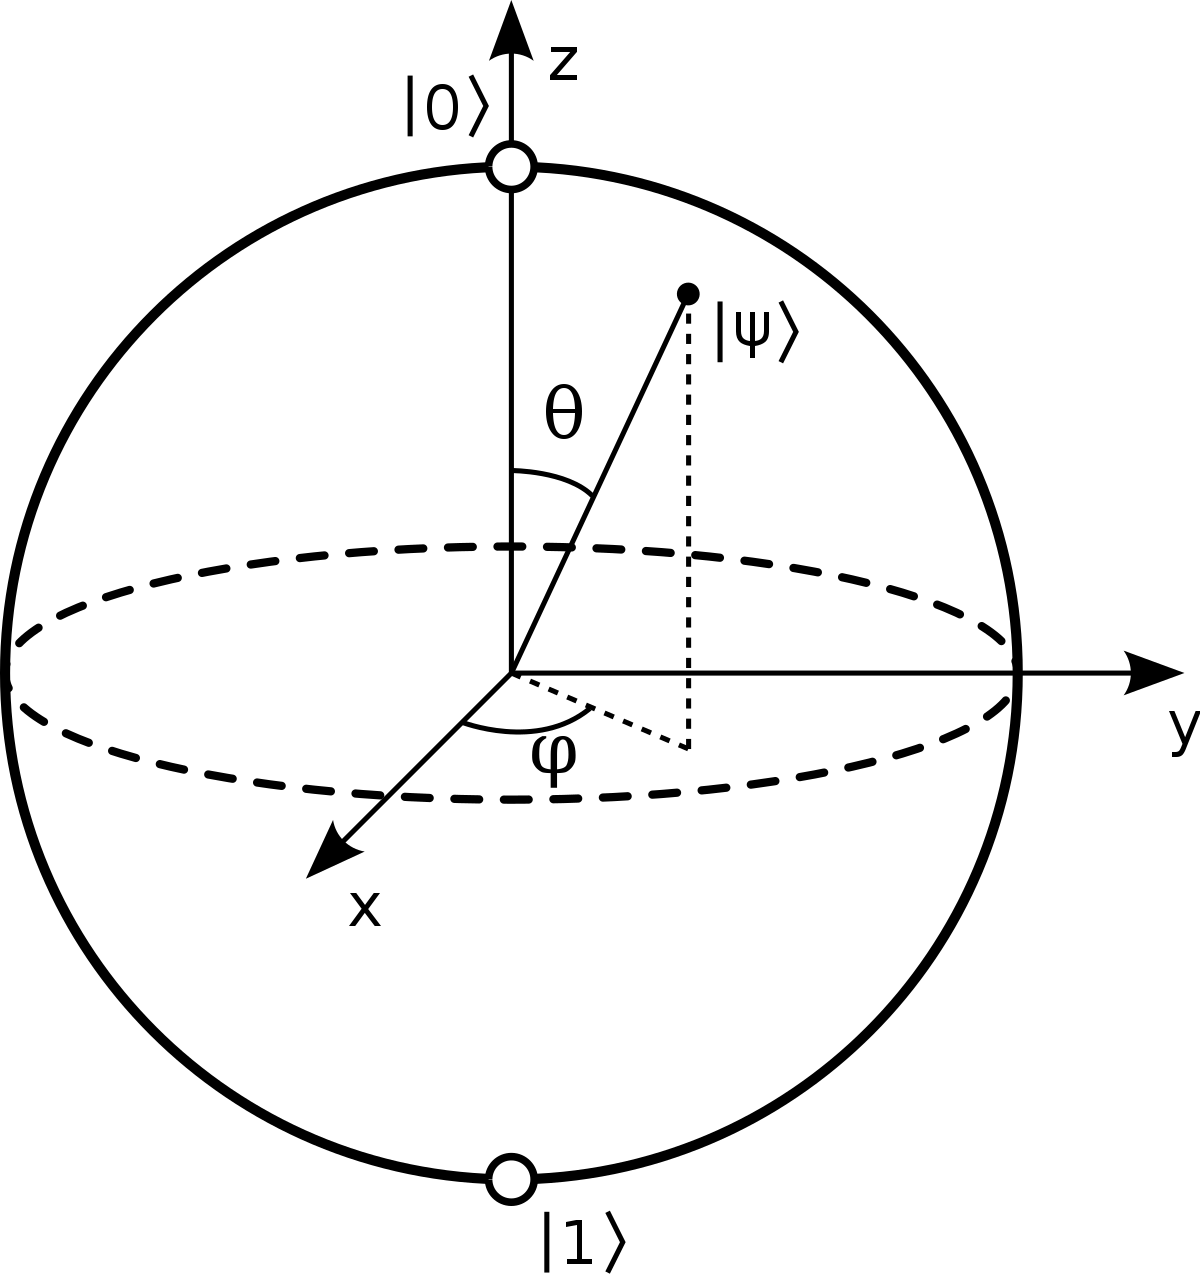
\includegraphics[width=0.5\textwidth]{figures/blochsphere.png}
        \end{subfigure}
        \begin{subfigure}{0.45\textwidth}
            \centering
            \begin{gather*}
                \begin{bmatrix}
                    c_{1,1} & c_{1,2} & \ldots & c_{1,2^n} \\
                    c_{2,1} & c_{2,2} & \ldots & c_{2,2^n} \\
                    \vdots & \ddots & \ddots & \vdots \\
                    c_{2^n,1} & c_{2^n,2} & \ldots & c_{2^n,2^n}
                \end{bmatrix}
            \end{gather*}
        \end{subfigure}
    \end{figure}

    The scale of computation is suddenly reduced. Instead of 40,000 dimension
    classical computation, we may only need \(\lceil{\log_2 (40000)}\rceil = 16\)
    qubit sized computation systems.

\end{frame}

% yes, vqas
\begin{frame}
    \frametitle{Quantum, sure, but NISQ?}

    In the near term, it seems the required number of qubits to outpace
    classical computers may not be out of reach. But can we reliably perform
    those computations on our quantum computers? Short coherence times make this
    impossible to do directly.

    Perhaps the constrained calculations can be processed as a subroutine? Yes,
    with \emph{Variational Quantum Algorithms}!

\end{frame}
